\section{Overview of \name}
\label{sec:overview}

To optimize inter-DC multicasts while minimizing
interference with latency-sensitive traffic, we present {\em \name},
a near-optimal inter-DC multicast overlay network.
Unlike previous designs which always, to some extent, keep
some local control capability at individual servers,
\name takes an explicit stance of {\em fully centralizing} the
control of the multicast overlay network.
Before presenting \name in more details,
we first highlight the intuitions behind its design
choice and the challenge to make it practical.


%\name is built on a couple of design choices, which
%trade marginal costs for substantial performance benefits.
%Before describing the details of \name's design, we first
%highlight the design choices and the intuition behind
%their cost-benefit tradeoffs
%(summarized in Table~\ref{tab:design-choices}).



%The insights obtained from \company's operational experience has inspired the design of \name, a near-optimal inter-DC multicast overlay network. This section starts with \name key design choices, highlights the design philosophy behind our choices, and provide an overview of the \name system, which builds on these design choices.

%\subsection{Why a fully centralized design}

\mypara{Conventional wisdom}
The limitations of many prior approaches~\cite{Andreev2013Designing,Repantis2010Scaling,Huang2014A}, including \company's
system, as highlighted in \Section\ref{subsec:motivation:baseline},
stem from suboptimal local adaptation decisions made by individual servers
in lack of global view and coordination.
These limitations remain, though to a lesser extent, in hybrid
control schemes (e.g.,~\cite{yin2009design,mukerjee2014enabling})
which combines real-time local adaptation with a centralized logic
operating on coarser timescales.
Despite these limitations, the
conventional wisdom has
been that local adaptation is needed to achieve desirable
scalability and responsiveness, and thus the cost of suboptimal
performance is deemed necessary.

\begin{figure}[t]
  \centering
  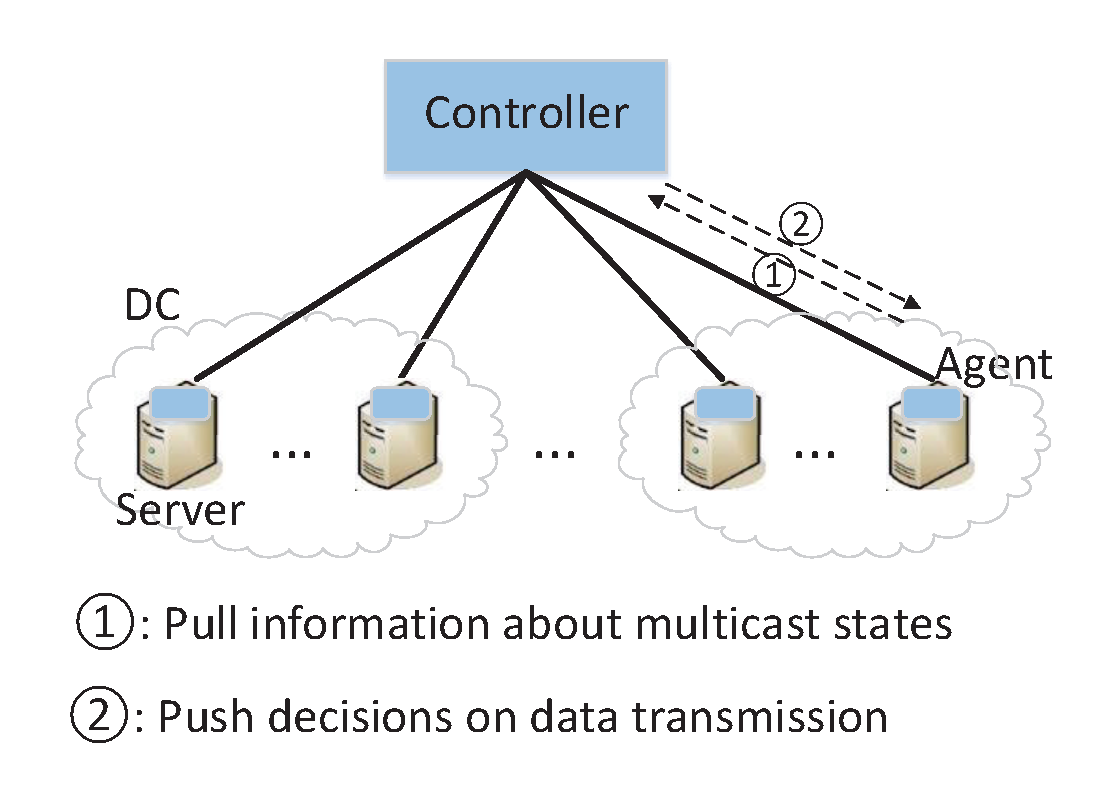
\includegraphics[width=2in]{images/framework.eps}
  \tightcaption{The centralized design of \name.}
  \label{fig:framework}
\vspace{-0.4cm}
\end{figure}

\mypara{Centralized design}
However, we believe that in the setting of inter-DC
multicasts, near-optimal performance can be achieved
through a fully centralized design.
As illustrated in Figure~\ref{fig:framework},
\name uses a centralized controller to update decisions,
including scheduling of data transfers, and the path selection and
bandwidth allocation of each transfer, on timescales of
several seconds.
At a high level, \name controller periodically pulls information
from all servers to maintain a most up-to-date global view of
multicast states, updates the decisions, and pushes them
to agents running locally on servers.
(That said, when the controller fails or is
not reachable, \name will fallback to a decentralized
overlay protocol to ensure graceful degradation on performance.)

%\mypara{Design philosophy}
Our centralized design is driven by four
considerations:
\begin{packedenumerate}
\item {\em Large data sizes:}
Sizes of inter-DC multicast are much larger
than those of online inter-DC traffic of interactive applications
(e.g., online partition-aggregation) and
traditional overlay networks (e.g., live streaming).
As a result, inter-DC multicast typically
last much longer than changes in
network conditions, so being highly responsive
to transient network dynamics is a secondary concern.
Instead, we can tolerate a small delay (of a few seconds)
to query a centralized controller.
The tradeoff between a centralized design and a decentralized one
in this context is that centralized control essentially trades
real-time responsiveness to network dynamics for
closer-to-optimal control decisions driven by
a global view of data delivery at each server.
\item {\em Large decision space:}
The sheer numbers of inter-DC overlay paths,
which grow exponentially with more servers acting as overlay nodes,
make it hard for individual servers to explore all possible overlay
paths based only on its local measurements.
Instead, there is a great room for improving overlay multicast
performance by maintaining a global view of data delivery states at
different servers in order to balance the availability across
different data blocks.
This turns out to be critical to achieving near-optimal performance
(\Section~\ref{sec:logic}).
\item {\em Need for strict traffic isolation:}
As observed in \Section\ref{subsec:motivation:baseline}, it is vital that inter-DC
multicast avoids hotspots and excessive use of
bandwidth, which could increase the latency of delay-sensitive traffic.
While it is difficult to enforce a limit on outgoing traffic
without any coordination across overlay servers, we found it is practical
to determine the bandwidth allocation and periodically update it
to all servers in a centralized fashion (\Section~\ref{sec:system}).
\item {\em Engineeringly simpler:}
In some sense, the resulting centralized system is conceptually
less complex than a decentralized/hybrid design
and amenable to a simple implementation.
The control logic running locally in each server
is only triggered on arrivals of new data units or control messages,
and thus can be stateless and lightweight.

\end{packedenumerate}

\mypara{Fast and near-optimal decision-making}
In essence, \name trades updating decisions on coarse timescales
for the potential of making optimal decisions in a centralized
fashion.
The key to striking such a favorable balance is a
near-optimal and efficient overlay routing
algorithm that can be updated on near-realtime timescales.
At a first glance, this is indeed intractable:
the centralized overlay routing algorithm must pick the next hops
from 10,000s servers for 100,000s objects, a scale that could
grow exponentially as we consider all possible
overlay paths that go through these servers and chop each data
object into many fine-grained blocks to send data simultaneously along
multipath overlay paths.
It is unclear how this problem can be solved even with
limited approximation, which was partly why \company has been lukewarm
about a centralized control architecture, despite its potential benefits.
The next section  will present how \name addresses this
challenge.

%The key technical challenge here is how to make optimal overlay scheduling and routing decisions at the scale tens of thousands of objects and tens of thousands of servers in near real time. To achieve desirable performance in a multicast overlay network, fully exploiting all the available overlay paths is essential, but it is untenable to go through all the potential servers and exponentially more paths by traditional approaches.

%\begin{itemize}
%
%\item Idea \#1: Fully centralized control
%
%\item Idea \#2: Dynamic bandwidth separation: separating background bulk data transfer from latency-sensitive traffic
%
%\item These ideas introduces performance costs (not real time, potentially low link utilization) are outweighed by benefits (not real time, potentially low link utilization)
%
%\item Design philosophy: the costs are outweighed by the benefits. (1) bulk data transfer can tolerate updates at coarse timescales. (2) the aggregation of latency-sensitive data is stable on timescales of several seconds. (3) the resulting system is amenable to simpler implementation.
%
%\item Key technical challenge: how to make optimal overlay scheduling and routing decisions at the scale tens of thousands of objects and tens of thousands of servers in near real time.
%
%\end{itemize}



